\appendix
\chapter{考前比记}

\begin{multicols}{3}
  \begin{itemize}
    \item \textbf{Prime Number $ < $ 100}: 2, 3, 5, 7, 11, 13, 17, 19, 23, 29,
    31, 37, 41, 43, 47, 53, 59, 61, 67, 71, 73, 79, 83, 89, 97

    \item \textbf{Simple Interest}
    \begin{equation}
      V = P \left( 1 + \frac{tr}{100} \right)
    \end{equation}

    \begin{itemize}
      \item $ P $: principal
      \item $ t $: time
      \item $ r $: interest rate
    \end{itemize}

    \item \textbf{Compound Interest}: $ t $ is years
    \begin{itemize}
      \item \textbf{Compounded Once Per Year}
      \begin{equation}
        V = P \left( 1 + \frac{r}{100} \right)^{t}
      \end{equation}

      \item \textbf{Compounded $ n $ Times Per Year}
      \begin{equation}
        V = P \left( 1 + \frac{r}{100n} \right)^{nt}
      \end{equation}
    \end{itemize}

    \item \textbf{图内三角形个数}
    \begin{equation}
      n - 2
    \end{equation}

    \item \textbf{边形的内角和公式}:
    \begin{equation}
      \left( n - 2 \right) \times 180
    \end{equation}

    \item \textbf{Congruent Triangle}
    \begin{itemize}
      \item 边边边
      \item 边角边
      \item 角边角
    \end{itemize}

    \item \textbf{Similar Triangle}:
    \begin{itemize}
      \item 两条边成比例, 夹角一样则相似
      \item \textbf{面积比为边长比的平方}
    \end{itemize}

    \item \textbf{Trapezoid (梯形) 面积}
    \begin{equation}
      S = \frac{1}{2}\left( b_{1} + b_{2} \right) \times h
    \end{equation}

    \item 当圆内接三角形有一边是直径的时候,该边对应的角为直角; 反之,当圆内接三角形有一
    个角为直角 时,该三角形必有一边为直径


  \end{itemize}
\end{multicols}

\section{3D 公式}

  \begin{figure}[H]
    \centering
    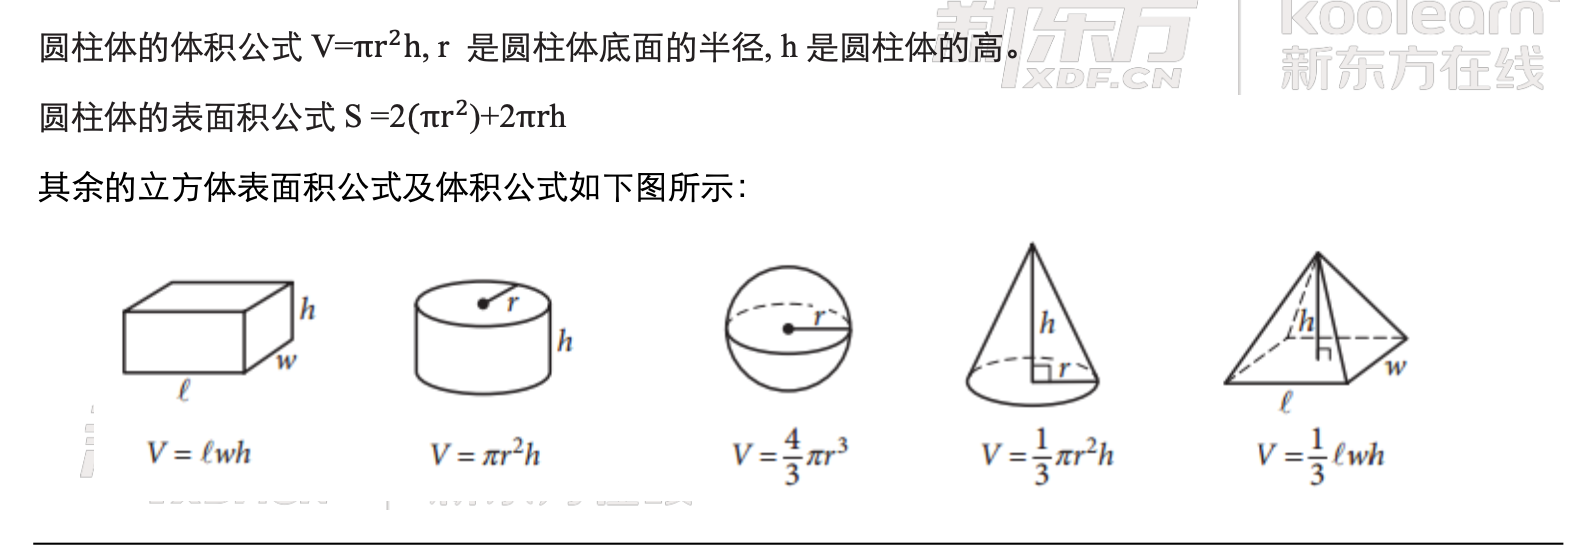
\includegraphics[width=\columnwidth]{images/remember-before-test/3d-equations.png}
  \end{figure}
